\documentclass[crop,border={20pt 20pt 20pt 20pt}]{standalone}
\usepackage{tikz,fontawesome5,fontspec,color}

\setmainfont{TeXGyreTermes}[
    Path = ../fonts/,
    UprightFont = *-Regular,
    BoldFont = *-Bold,
    ItalicFont = *-Italic,
    BoldItalicFont = *-BoldItalic]

\definecolor{concept}{HTML}{ECEFF1}
\definecolor{prior}{HTML}{E6EE9C}
\definecolor{paper}{HTML}{BBDEFB}

\newcommand{\op}{\textnormal{\scalebox{.65}{\faChartLine}}}
\newcommand{\vi}{\textnormal{\scalebox{.65}{\faShield*}}}
\newcommand{\fm}{\textnormal{\scalebox{.65}{\faCheck}}}
\newcommand{\pa}{\textnormal{\scalebox{.65}{\faCode}}}

\tikzstyle{start} = [rectangle, 
  minimum width=7cm,
  minimum height=1.8cm,
  text width=7cm, 
  text centered,  
  draw=black, 
  densely dashed,
  fill=concept]
\tikzstyle{prior} = [start, solid, fill=prior, minimum height=2cm]
\tikzstyle{node} = [prior, fill=paper]
\tikzstyle{arrow} = [thick,->,>=stealth]
\tikzstyle{rectangle connector} = [thick,->,>=stealth,pos=0.5, to path={(\tikztostart) -- ++(#1,0pt) \tikztonodes |- (\tikztotarget)}]
\tikzstyle{topic icon} = [rectangle, text width=.5cm, yshift=2.3cm]
\tikzstyle{topic label} = [rectangle, text width=5cm, yshift=-.25mm]

\begin{document}
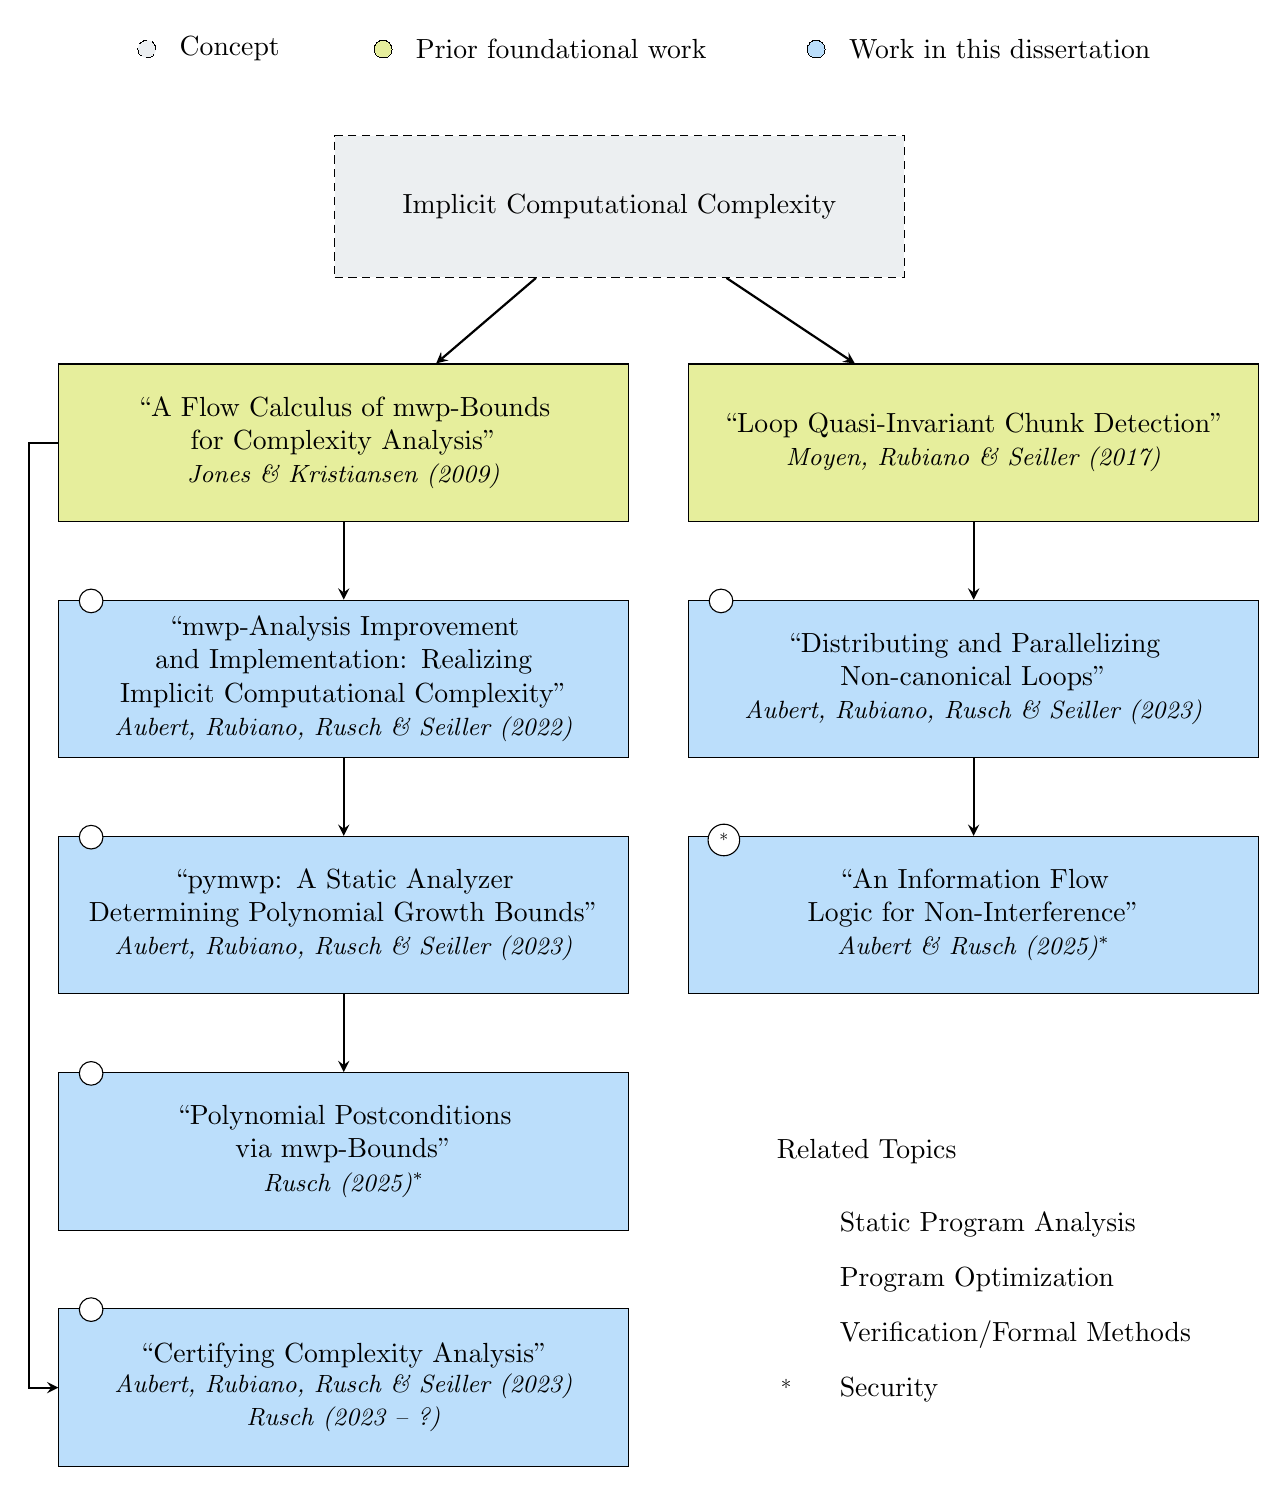
\begin{tikzpicture}[node distance=3cm,
	block/.style args={#1:#2:#3}{node, 
	name={#1}, draw,
    node contents={#3},
    append after command={
    	node[circle, fill=white, draw=black, solid,
        minimum size=3mm, inner sep=2pt, outer sep=0.4pt, xshift=3mm, yshift=1mm,
        anchor=north west]
        at (#1.north west) {#2}}}]
    
\fill[line width=0mm, fill=concept, draw=black, densely dashed] (-6, 0) circle (.75ex) node[right, xshift=3mm]{Concept};
\fill[line width=0mm, fill=prior, draw=black] (-3, 0) circle (.75ex) node[right, xshift=3mm]{Prior foundational work};
\fill[line width=0mm, fill=paper, draw=black] (2.5, 0) circle (.75ex) node[right, xshift=3mm]{Work in this dissertation};

\node (icc) [start, yshift=-2cm] {Implicit Computational Complexity};
\node (mwp) [prior, below of=icc, xshift=-3.5cm] {``A Flow Calculus of mwp-Bounds\\for Complexity Analysis"\\\small{\textit{Jones \& Kristiansen (2009)}}};
\node (qsi) [prior, right of=mwp, xshift=5cm] {``Loop Quasi-Invariant Chunk Detection"\\\small{\textit{Moyen, Rubiano \& Seiller (2017)}}};
\node [block=imp:\pa:{``mwp-Analysis Improvement and Implementation: Realizing\\Implicit Computational Complexity"\\\small{\textit{Aubert, Rubiano, Rusch \& Seiller (2022)}}}, below of=mwp];
\node [block=pym:\pa:{``pymwp: A Static Analyzer\\Determining Polynomial Growth Bounds"\\\small{\textit{Aubert, Rubiano, Rusch \& Seiller (2023)}}}, below of=imp];
\node [block=pci:\fm:{``Polynomial Postconditions\\via mwp-Bounds"\\\small{\textit{Rusch (2025)$^*$}}}, below of=pym];
\node [block=ncl:\op:{``Distributing and Parallelizing\\Non-canonical Loops"\\\small{\textit{Aubert, Rubiano, Rusch \& Seiller (2023)}}}, below of=qsi];
\node [block=nil:\vi:{``An Information Flow Logic for Non-Interference"\\\small{\textit{Aubert \& Rusch (2025)$^*$}}}, below of=ncl];
\node [block=cca:\fm:{``Certifying Complexity Analysis"\\\small{\textit{Aubert, Rubiano, Rusch \& Seiller (2023)}}\\\small{\textit{Rusch (2023 -- ?)}}}, below of=pci];

\draw [arrow] (icc) -- (mwp);
\draw [arrow] (mwp) -- (imp);
\draw [arrow] (imp) -- (pym);
\draw [arrow] (pym) -- (pci);
\draw [arrow] (icc) -- (qsi); 
\draw [arrow] (qsi) -- (ncl); 
\draw [arrow] (ncl) -- (nil); 
\draw [rectangle connector=-4cm] (mwp) to (cca);

\node (topics)   [rectangle, below of=nil, text width=5cm] {Related Topics};
\node (analysis) [topic icon, xshift=-2.2cm, yshift=-.2cm, below of=topics] {\large\pa};
\node            [topic label, right of=analysis] {Static Program Analysis};
\node (optimize) [topic icon, below of=analysis] {\large\op};
\node            [topic label, right of=optimize] {Program Optimization};
\node (verify)   [topic icon, below of=optimize] {\large\fm};
\node            [topic label, right of=verify] {Verification/Formal Methods};
\node (security) [topic icon, below of=verify] {\large\vi};
\node          	 [topic label, right of=security] {Security};

\end{tikzpicture}
\end{document}